\chapter{Experiments with Two Conditions}
\makeheading{Week 2}
\section*{Anatomy of an A/B Test}
\begin{itemize}
      \item One design factor at two levels.
      \item We now consider the design and analysis of an experiment
            consisting of two experimental conditions --- or what many
            data scientists broadly refer to as ``A/B Testing''
            which is synonymous with ``experimentation''
            in data science.
            \begin{itemize}
                  \item Canonical A/B test:
                        \begin{figure}[!htbp]
                              \centering
                              
\begin{tikzpicture}[x=0.75pt,y=0.75pt,yscale=-1.5,xscale=1.5]
                                    %Rounded Rect [id:dp8976617722511913] 
                                    \draw  [draw opacity=0][fill={rgb, 255:red, 208; green, 2; blue, 27 }  ,fill opacity=1 ] (10,19.53) .. controls (10,15.12) and (13.58,11.53) .. (18,11.53) -- (81.3,11.53) .. controls (85.72,11.53) and (89.3,15.12) .. (89.3,19.53) -- (89.3,43.53) .. controls (89.3,47.95) and (85.72,51.53) .. (81.3,51.53) -- (18,51.53) .. controls (13.58,51.53) and (10,47.95) .. (10,43.53) -- cycle ;
                                    %Rounded Rect [id:dp05576705853009267] 
                                    \draw  [draw opacity=0][fill={rgb, 255:red, 74; green, 144; blue, 226 }  ,fill opacity=1 ] (102,19.07) .. controls (102,14.65) and (105.58,11.07) .. (110,11.07) -- (173.3,11.07) .. controls (177.72,11.07) and (181.3,14.65) .. (181.3,19.07) -- (181.3,43.07) .. controls (181.3,47.48) and (177.72,51.07) .. (173.3,51.07) -- (110,51.07) .. controls (105.58,51.07) and (102,47.48) .. (102,43.07) -- cycle ;
                                    % Text Node
                                    \draw (49.65,31.53) node  [color={rgb, 255:red, 255; green, 255; blue, 255 }  ,opacity=1 ] [align=left] {CLICK ME};
                                    % Text Node
                                    \draw (141.65,31.07) node  [color={rgb, 255:red, 255; green, 255; blue, 255 }  ,opacity=1 ] [align=left] {CLICK ME};
                              \end{tikzpicture}
                              \caption{Button-Colour Experiment}
                        \end{figure}

                        Here, the metric of interest might be click-through-rate, which
                        we're interested in maximizing.
            \end{itemize}
      \item Other, more tangible examples:
            \begin{itemize}
                  \item Amazon
                        \begin{itemize}
                              \item Checkout reassurances
                              \item List view vs.\ tile view
                        \end{itemize}
                  \item Airbnb
                        \begin{itemize}
                              \item Host landing page redesign
                              \item Next available date
                        \end{itemize}
            \end{itemize}
      \item Typically, the goal of such an experiment is to decide which condition is optimal
            with respect to some metric of interest $ \theta $. This could be a
            \begin{itemize}
                  \item mean (e.g., average time on page, average purchase size, average revenue per customer)
                  \item proportion (e.g., CTR, bounce rate, retention rate)
                  \item variance
                  \item quantile (e.g., median, $ 95^{\text{th}} $ percentile of page load time)
                  \item technically any statistic that can be from sample data
            \end{itemize}
      \item Consider the button-colour example: imagine the observed click-through-rates (CTR) of the two
            conditions are: $ \hat{\theta}_1=0.12 $ (red) and $ \hat{\theta}_2=0.03 $ (blue).
            \begin{itemize}
                  \item Obviously, $ \hat{\theta}_1>\hat{\theta}_2 $, but does that mean that
                        $ \theta_1>\theta_2 $?
            \end{itemize}
      \item Formally, such a question is phrased as a statistical hypothesis that we test using
            the data collected from the experiment.
            \begin{itemize}
                  \item $ H_0 $: $ \theta_1=\theta_2 $ versus $ H_\text{A} $: $ \theta_1\ne\theta_2 $ (two-sided).
                  \item $ H_0 $: $ \theta_1\le\theta_2 $ versus $ H_\text{A} $: $ \theta_1>\theta_2 $ (one-sided).
                  \item $ H_0 $: $ \theta_1\ge\theta_2 $ versus $ H_\text{A} $: $ \theta_1<\theta_2 $ (one-sided).
            \end{itemize}
      \item ``Absence of evidence $ \ne  $ evidence of absence.''
      \item No matter which hypothesis is appropriate, the goal is always the same: based on the
            observed data, we will decide to \emph{reject} $ H_0 $ or \emph{not reject} $ H_0 $.
      \item In order to draw such a conclusion, we will define a \textbf{test statistic} $ T $,
            which is a random variable that satisfies three properties:
            \begin{enumerate}[(i)]
                  \item It must be a function of the observed data.
                  \item It must be a function of the parameters $ \theta_1 $ and $ \theta_2 $.
                  \item Its distribution must not depend on $ \theta_1 $ or $ \theta_2 $.
            \end{enumerate}
      \item Assuming the null hypothesis is true, the test statistic $ T $ follows
            a particular distribution which we call the \textbf{null distribution}.
            For example, $ \N{0,1} $, $ t(\texttt{df}) $,
            $ F(\texttt{df1}, \texttt{df2}) $, $ \chi^2(\texttt{df}) $.
      \item We then calculate $ t $, the observed value of the test statistic, and evaluate its extremity
            relative to the null distribution.
            \begin{itemize}
                  \item If $ t $ is very extreme, this suggests that perhaps the null hypothesis
                        is not true.
                  \item If $ t $ appears as though it could have come from the null distribution, then
                        there is no reason to disbelieve the null hypothesis.
            \end{itemize}
      \item We formalize the extremity of $ t $ using the \textbf{$ \symbf{p} $-value} of the test.

            \begin{Definition}{$ \symbf{p} $-value}{}
                  The probability of observing a value of the test statistic \emph{at least as extreme}
                  as the value we observed, if the null hypothesis is true.
            \end{Definition}
            \begin{itemize}
                  \item Thus, the $ p $-value formally quantifies how ``extreme'' the observed
                        test statistic is.
                  \item The more extreme the value of $ t $, the smaller the $ p $-value, and the more
                        evidence we have against it.
            \end{itemize}
      \item How ``extreme'' $ t $ must be, and hence how small the $ p $-value must be
            to reject $ H_0 $, is determined by the \textbf{significance level} of the test,
            denoted $ \alpha $.
            \begin{itemize}
                  \item If $ p $-value $ \le \alpha $, we reject $ H_0 $.
                  \item If $ p $-value $ >\alpha $, we do not reject $ H_0 $.
                        \begin{Remark}{}{}
                              Common choices of $ \alpha $ are $ 0.05 $ and $ 0.01 $.
                        \end{Remark}
            \end{itemize}
      \item In order to choose $ \alpha $, one must understand the two types of errors
            that can be made when drawing conclusion in the context of a hypothesis test.
      \item Recall that by design, either $ H_0 $ or $ H_{\text{A}} $ is true.
            Thus means that there are four possible outcomes when using data to decide which
            statement is true:
            \begin{enumerate}[(1)]
                  \item No Error: $ H_0 $ is true, and we correctly do not reject it.
                  \item Type I Error: $ H_0 $ is true, and we incorrectly reject it.
                  \item Type II Error: $ H_0 $ is false, and we incorrectly do not reject it.
                  \item No Error: $ H_0 $ is false, and we correctly reject it.
            \end{enumerate}
      \item We would like to reduce the likelihood of making either type of error.
            \begin{itemize}
                  \item But there are different consequences of each type of error.
                  \item So we may wish to treat them differently.
            \end{itemize}
\end{itemize}
\begin{Example}{Pregnancy Test}{}
      \centerline{$ H_0 $: person is not pregnant versus $ H_\text{A} $: person is pregnant.}
      \begin{itemize}
            \item Type I Error: person is pregnant (false positive).
            \item Type II Error: person is not pregnant (false negative).
      \end{itemize}
\end{Example}
\begin{Example}{Courtroom}{}
      \centerline{$ H_0 $: the defendant is innocent versus $ H_\text{A} $: the defendant is guilty.}
      \begin{itemize}
            \item Type I Error: sentencing an innocent person to jail.
            \item Type II Error: letting a guilty person go free.
      \end{itemize}
\end{Example}
\begin{itemize}
      \item $ \alpha=\Prob*{\text{Type I Error}} $.
      \item $ \beta=\Prob*{\text{Type II Error}} $
            where $ 1-\beta=\text{Power} $.
      \item Fortunately, it is possible to control the frequency in which these types of errors
            occur.
      \item It is desirable to have a test with a small significance level, and a large power.
\end{itemize}
\section{Comparing Means in Two Conditions}
\begin{itemize}
      \item Here, we restrict attention to the situation in which the response variable
            of interest is measured on a continuous scale.
      \item We assume that the response observations collected in the two conditions follow normal
            distributions, and in particular
            \[ Y_{i1}\sim \N{\mu_1,\sigma^2}\text{ and }Y_{i2} \sim \N{\mu_2,\sigma^2},\quad i=1,2,\ldots,n_j\text{ for } j=1,2. \]
            \begin{itemize}
                  \item $ Y_{ij}= $ response observation for unit $ i $ in condition $ j $.
            \end{itemize}
      \item Using the observed data, we test hypotheses of the form:
            \begin{itemize}
                  \item $ H_0 $: $ \mu_1=\mu_2 $ versus $ H_\text{A} $: $ \mu_1\ne\mu_2 $.
                  \item $ H_0 $: $ \mu_1\le\mu_2 $ versus $ H_\text{A} $: $ \mu_1>\mu_2 $.
                  \item $ H_0 $: $ \mu_1\ge\mu_2 $ versus $ H_\text{A} $: $ \mu_1<\mu_2 $.
            \end{itemize}
\end{itemize}
\subsection{The Two-Sample \texorpdfstring{$ t $}{t}-Test}
\begin{Statistical_Test}{Student's $ \symbf{t} $-test}{st_t_test}
      \begin{itemize}
            \item \emph{Purpose}: Compare $ \mu_1 $ versus $ \mu_2 $ (assuming $ \sigma_1=\sigma_2 $ are unknown).
            \item \emph{Test Statistic}:
                  \[ T=\frac{\bigl(\bar{Y}_1-\bar{Y}_2\bigr)-\overbracket{(\mu_1-\mu_2)}^0}{\displaystyle \hat{\sigma}\sqrt{\frac{1}{n_1}+\frac{1}{n_2}}}\sim t(n_1+n_2-2) \]
                  \begin{itemize}
                        \item $ \hat{\sigma} $ is our estimator.
                        \item $ t(n_1+n_2-2) $ is our null distribution.
                  \end{itemize}
            \item \emph{Observed Version}:
                  \[ t=\frac{\bigl(\bar{y}_1-\bar{y}_2\bigr)-0}{\displaystyle \hat{\sigma}\sqrt{\frac{1}{n_1}+\frac{1}{n_2}}}
                        =\frac{\hat{\mu}_1-\hat{\mu}_2}{\displaystyle \hat{\sigma}\sqrt{\frac{1}{n_1}+\frac{1}{n_2}}} \]
                  \begin{itemize}
                        \item $ \displaystyle \bar{y}_j= \frac{1}{n_j}\sum_{i=1}^{n_j} y_{ij}=\hat{\mu}_j $.
                        \item $ \displaystyle \hat{\sigma}^2=\frac{(n_1-1)\hat{\sigma}_1^2+(n_2-1)\hat{\sigma}_2^2}{n_1+n_2-2} $.
                        \item $ \displaystyle \hat{\sigma}_j^2=\frac{1}{n_j-1} \sum_{i=1}^{n_j} \bigl(y_{ij}-\bar{y}_j\bigr)^2 $.
                  \end{itemize}
            \item \emph{$ p $-value Calculation}:
                  \begin{itemize}
                        \item For $ H_0 $: $ \mu_1=\mu_2 $ versus $ H_\text{A} $: $ \mu_1\ne\mu_2 $, we compute
                              $ p\text{-value}=\Prob*{T\ge \abs{t}}+\Prob*{T\le -\abs{t}} $.
                        \item For $ H_0 $: $ \mu_1\le\mu_2 $ versus $ H_\text{A} $: $ \mu_1>\mu_2 $, we compute
                              $ p\text{-value}=\Prob*{T\ge t} $.
                        \item For $ H_0 $: $ \mu_1\ge\mu_2 $ versus $ H_\text{A} $: $ \mu_1<\mu_2 $, we compute
                              $ p\text{-value}=\Prob*{T\le t} $.
                  \end{itemize}
                  \begin{Remark}{}{}
                        In all cases above, $ T \sim t(n_1+n_2-2) $.
                  \end{Remark}
      \end{itemize}
\end{Statistical_Test}
\subsection{When Assumptions are Invalid}
\begin{Statistical_Test}{Welch's $ \symbf{t} $-test}{}
      \begin{itemize}
            \item \emph{Purpose}: Compare $ \mu_1 $ versus $ \mu_2 $ (assuming $ \sigma_1\ne\sigma_2 $ are unknown).
            \item \emph{Test Statistic}: ``Approximately,'' we have
                  \[ T=\frac{\bigl(\bar{Y}_1-\bar{Y}_2\bigr)-\overbracket{(\mu_1-\mu_2)}^0}{\displaystyle \sqrt{\frac{\hat{\sigma}_1^2}{n_1}+\frac{\hat{\sigma}_2^2}{n_2}}}\stackrel{\cdot}{\sim} t(\nu) \]
                  where
                  \[ \nu=\frac{
                              \displaystyle \biggl(\frac{\hat{\sigma}_1^2}{n_1}+\frac{\hat{\sigma}_2^2}{n_2} \biggr)^{\!2}
                        }{
                              \displaystyle \frac{(\hat{\sigma}_1^2/n_1)^2}{n_1-1}+\frac{(\hat{\sigma}_2^2/n_2)^2}{n_2}
                        }\approx \min(n_1,n_2)-1  \]
            \item \emph{Observed Version}:
                  \[ t=\frac{\bigl(\bar{y}_1-\bar{y}_2\bigr)-0}{\displaystyle \sqrt{\frac{\hat{\sigma}_1^2}{n_1}+\frac{\hat{\sigma}_2^2}{n_2}}}=\frac{\hat{\mu}_1-\hat{\mu}_2}{\displaystyle \sqrt{\frac{\hat{\sigma}_1^2}{n_1}+\frac{\hat{\sigma}_2^2}{n_2}}}  \]
            \item \emph{$ p $-value Calculation}: Same as~\Cref{stest:st_t_test}, but where
                  the null distribution is $ T \sim t(\nu) $.
      \end{itemize}
\end{Statistical_Test}
\begin{Statistical_Test}{$ \symbf{F} $-test for Variances}{}
      \begin{itemize}
            \item \emph{Purpose}:
                  \begin{itemize}
                        \item $ H_0 $: $ \sigma_1^2=\sigma_2^2 $ versus $ H_\text{A} $: $ \sigma_1^2\ne \sigma_2^2 $.
                        \item $ H_0 $: $ \sigma_1^2/\sigma_2^2=1 $ versus $ H_\text{A} $: $ \sigma_1^2/\sigma_2^2\ne 1 $.
                  \end{itemize}
            \item \emph{Test Statistic}:
                  \[ T=\frac{\hat{\sigma}_1^2}{\hat{\sigma}_2^2}\sim F(n_1-1,n_2-1)  \]
            \item \emph{Observed Version}:
                  \[ t=\frac{\hat{\sigma}_1^2}{\hat{\sigma}_2^2}\in\mathbf{R}   \]
            \item \emph{$ p $-value Calculation}:
                  \begin{itemize}
                        \item If $ t\ge 1 $, then $ p\text{-value}=\Prob*{T\ge t}+\Prob*{T\le 1/t} $.
                        \item If $ t<1 $, then $ p\text{-value}=\Prob*{T\le t}+\Prob*{T\ge 1/t} $.
                  \end{itemize}
                  \begin{Remark}{}{}
                        In all cases above, $ T \sim F(n_1-1,n_2-1) $.
                  \end{Remark}
      \end{itemize}
\end{Statistical_Test}
\subsection{Example: Instagram Ad Frequency}
\begin{Example}{Instagram Ad frequency}{}
      \begin{itemize}
            \item Suppose that you are a data scientist at Instagram, and you are interested
                  in running an experiment to learn about how user engagement is influenced by ad frequency.
            \item Currently, users see an ad every 8 posts in their social feed, but, in order
                  to increase ad revenue, your manager is pressuring your team to show an ad every 5 posts.
                  \begin{itemize}
                        \item Condition 1: 7:1 Ad Frequency
                        \item Condition 2: 4:1 Ad Frequency
                  \end{itemize}
            \item You are justifiably nervous about this change, and you worry that this
                  will substantially decrease user engagement and hurt the overall user experience.
            \item The metric of interest you choose to optimize for is $ \mu=\text{average session time} $
                  (where $ y =$ the length of time a user engages within the app, in minutes).
            \item The hypothesis being tested here is:

                  \centerline{$ H_0 $: $ \mu_1\le \mu_2 $ versus $ H_\text{A} $: $ \mu_1>\mu_2 $}
            \item The data summaries are:
                  \begin{itemize}
                        \item $ n_1=500 $, $ \hat{\mu}_1=\bar{y}_1=4.92 $, $ \hat{\sigma}_1=s_1=0.96 $.
                        \item $ n_2=500 $, $ \hat{\mu}_2=\bar{y}_2=3.05 $, $ \hat{\sigma}_2=s_2=0.99 $.
                  \end{itemize}
      \end{itemize}
      \begin{framed}
            $ F $-test:
            \begin{itemize}
                  \item $ t=\hat{\sigma}_1^2/\hat{\sigma}_2^2=0.96^2/0.99^2=0.938 $.
                  \item $ p\text{-value}=\Prob*{T\le 0.938}+\Prob*{T\ge 1/0.938}=0.4720 $
                        where $ T \sim F(499,499) $.
                  \item This $ p $-value is larger than any ordinary $ \alpha $, so
                        we do not reject $ H_0 $: $ \sigma_1^2=\sigma_2^2 $, and so we continue
                        with Student's $ t $-test.
            \end{itemize}
      \end{framed}
      \begin{framed}
            Student's $ t $-test:
            \begin{itemize}
                  \item $ \displaystyle \hat{\sigma}^2=\frac{499(0.96)^2+499(0.99)^2}{998}=0.9793^2 $.
                  \item $ \displaystyle t=\frac{4.92-3.05}{0.9793\sqrt{\frac{1}{500} +\frac{1}{500} }}=30.1  $.
                  \item $ p\text{-value}=\Prob*{T\ge 30.1}=1.84\times 10^{-142}\approx 0 $ where $ T \sim t(998) $.
                  \item This $ p $-value is much smaller than any typical $ \alpha $, and so we reject
                        $ H_0 $: $ \mu_1\le \mu_2 $, and conclude that increasing ad frequency significantly
                        reduces average session duration.
            \end{itemize}
      \end{framed}
      \href{https://github.com/Hextical/university-notes/blob/master/year-3/semester-3/STAT 430/code/2.2 - Comparing_two_means.R}{[R Code] \texttt{Comparing\_two\_means}}
\end{Example}
\section{Comparing Proportions in Two Conditions}
\begin{itemize}
      \item Here, we restrict attention to the situation in which the response variable of interest
            is binary, indicating whether an experimental unit did, or did not, perform
            some action of interest. In cases like these, we let
            \[ Y_{ij}=\begin{cases*}
                        1 & if unit $ i $ in condition $ j $ performs the action of interest         \\
                        0 & if unit $ i $ in condition $ j $ does not perform the action of interest
                  \end{cases*}\quad i=1,2,\ldots,n_j\text{ for } j=1,2. \]
      \item Because the $ Y_{ij} $'s are binary, it is common to assume that they follow
            a Bernoulli distribution; that is, $ Y_{ij}\sim \bin{1,\pi_j} $ where
            $ \pi_j $ represents the probability that $ Y_{ij}=1 $. That is,
            the probability that unit $ i $ from condition $ j $ performs the ``action of interest.''
      \item Using the observed data, we test hypotheses of the form:
            \begin{itemize}
                  \item $ H_0 $: $ \pi_1=\pi_2 $ versus $ H_\text{A} $: $ \pi_1\ne\pi_2 $.
                  \item $ H_0 $: $ \pi_1\le\pi_2 $ versus $ H_\text{A} $: $ \pi_1>\pi_2 $.
                  \item $ H_0 $: $ \pi_1\ge\pi_2 $ versus $ H_\text{A} $: $ \pi_1<\pi_2 $.
            \end{itemize}
\end{itemize}
\subsection{\texorpdfstring{$ Z $}{Z}-tests for Proportions}
\begin{Statistical_Test}{$ \symbf{Z} $-test for Proportions}{}
      \begin{itemize}
            \item \emph{Purpose}: Compare $ \pi_1 $ versus $ \pi_2 $.
            \item \emph{Test Statistic}: ``Approximately,'' we have
                  \[ T=\frac{\bigl(\bar{Y}_1-\bar{Y}_2\bigr)-
                              \overbracket{(\pi_1-\pi_2)}^0}{\displaystyle \sqrt{\hat{\pi}(1-\hat{\pi})\biggl(\frac{1}{n_1} +\frac{1}{n_2} \biggr)}}\stackrel{\cdot}{\sim}\N{0,1} \]
                  where $ \displaystyle \hat{\pi}=\frac{n\hat{\pi}_1+n_2\hat{\pi}_2}{n_1+n_2}=\frac{\text{\# units who performed action}}{\text{total \# units in exp.}} $
                  and $ \hat{\pi}_j=\bar{y}_j $.
            \item \emph{Observed Version}:
                  \[ t=\frac{\bigl(\bar{y}_1-\bar{y}_2\bigr)-0}{\displaystyle \sqrt{\hat{\pi}(1-\hat{\pi})\biggl(\frac{1}{n_1} +\frac{1}{n_2} \biggr)}}=
                        \frac{\hat{\pi}_1-\hat{\pi}_2}{\displaystyle \sqrt{\hat{\pi}(1-\hat{\pi})\biggl(\frac{1}{n_1} +\frac{1}{n_2} \biggr)}}\]
            \item \emph{$ p $-value Calculation}: The $ p $-values are calculated
                  in the same way as in the $ t $-tests, except here that $ T \sim \N{0,1} $.
      \end{itemize}
\end{Statistical_Test}
\subsection{Example: Optimizing Optimizely}
\begin{Example}{Optimizing Optimizely}{optimizely_ex1}
      \begin{itemize}
            \item During a website redesign, Optimizely was interested in how new versions
                  of certain pages influenced things like conversion and engagement relative to the old version.
            \item One outcome they were interested in was whether the redesigned homepage lead to
                  a significant increase in the number of new accounts created.
                  \begin{itemize}
                        \item Condition 1: original homepage.
                        \item Condition 2: redesigned homepage.
                  \end{itemize}
            \item The metric of interest here is $ \pi= $ conversion rate (where $ y=1 $ if a homepage
                  visitor signed up and $ 0 $ otherwise).
            \item The hypothesis tested here is:

                  \centerline{$ H_0 $: $ \pi_1\ge \pi_2 $ versus $ H_\text{A} $: $ \pi_1<\pi_2 $}
            \item The data from this experiment may be summarized in a $ 2\times 2 $ contingency table:
                  \begin{center}
                        \begin{tabularx}{0.75\linewidth}{@{}BYYYY@{}}
                              \multicolumn{2}{c}{}        & \multicolumn{2}{c}{\textbf{Condition}} &                                                                                       \\
                              \multicolumn{2}{c}{}        & 1                                      & 2                          & \multicolumn{1}{c}{}                                     \\
                              \cmidrule{2-5}
                              \multirow{2}{*}{Conversion} & Yes                                    & $280$                      & $399$                      & $679$                       \\
                                                          & No                                     & $8592$                     & $8243$                     & $16835$                     \\
                              \cmidrule{2-5}
                              \multicolumn{1}{c}{}        & \multicolumn{1}{c}{}                   & \multicolumn{1}{c}{$8872$} & \multicolumn{1}{c}{$8642$} & \multicolumn{1}{c}{$17514$} \\
                        \end{tabularx}
                  \end{center}
            \item $ \hat{\pi}_1=280/8872=0.0316 $ and $ \hat{\pi}_2=399/8642=0.0462 $. Thus,
                  \[ \hat{\pi}=\frac{8872(0.0316)+8642(0.0462)}{17514} \]
                  \[ t=\frac{0.0316-0.0462}{\sqrt{(0.0388)(1-0.0388)(1/8872+1/8642)}}=-5.002  \]
            \item $ p\text{-value}=\Prob*{T\le -5.002}=2.84\times 10^{-7}\approx 0 $ where $ T \sim \N{0,1} $.
            \item We reject $ H_0 $ and conclude that the redesigned homepage significantly
                  increases conversion rate.
            \item \href{https://github.com/Hextical/university-notes/blob/master/year-3/semester-3/STAT 430/code/2.3 - Comparing_two_proportions.R}{[R Code] \texttt{Comparing\_two\_proportions}}
      \end{itemize}
\end{Example}
\section{Power Analysis and Sample Size Calculations}
\begin{itemize}
      \item Used to control Type II Error.
      \item Power analyses help determine required sample sizes.
      \item Suppose, for illustration, that we are interested in testing the hypothesis:

            \centerline{$ H_0 $: $ \theta_1=\theta_2 $ versus $ H_\text{A} $: $ \theta_1\ne \theta_2 $}
      \item Suppose, also for illustration, that the test statistic associated with this test has
            the form:
            \[ T=\frac{\bigl(\bar{Y}_1-\bar{Y}_2\bigr)-\overbracket{(\theta_1-\theta_2)}^0}{\displaystyle \sqrt{\frac{\Var{Y_1}}{n}+\frac{\Var{Y_2}}{n} }}\sim \N{0,1}  \]
      \item It will be useful to define the notion of a \textbf{rejection region}, denoted $ \mathcal{R} $,
            which is all the values of the observed test statistic $ t $ that would lead to the rejection
            of $ H_0 $:
            \[ \mathcal{R}=\set*{t\mid H_0\text{ is rejected}} \]
            \begin{itemize}
                  \item If $ t\in\mathcal{R} $, we reject $ H_0 $.
                  \item If $ t\in\mathcal{R}^c $, we do not reject $ H_0 $.
            \end{itemize}
            \begin{figure}[!htbp]
                  \centering
                  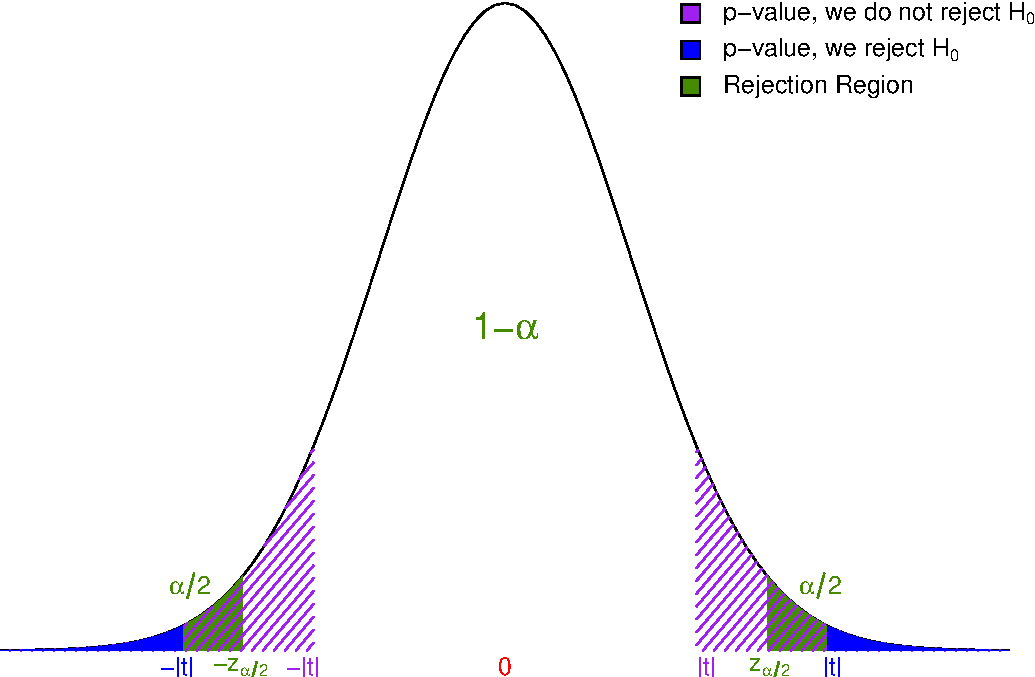
\includegraphics[width=0.5\textwidth]{1.pdf}
                  \caption{$ H_0 $: $ \theta_1=\theta_2 $ versus $ H_\text{A} $: $ \theta_1\ne \theta_2 $}{$ \mathcal{R}=\set{t\mid t\le -z_{\alpha/2}\text{ or }t\ge z_{\alpha/2}} $}
            \end{figure}
            \begin{figure}[!htbp]
                  \centering
                  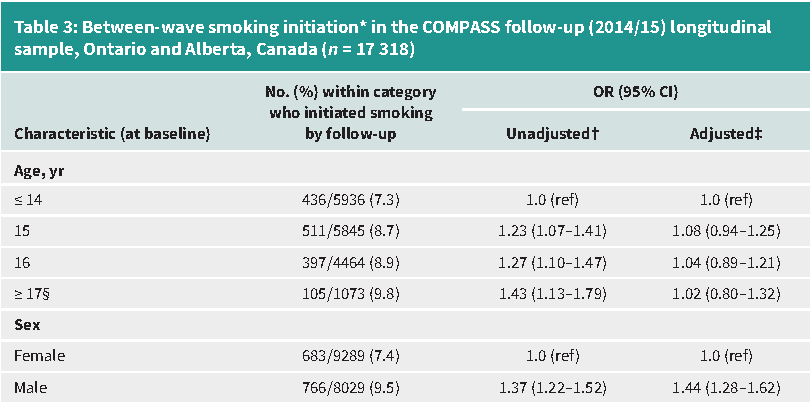
\includegraphics[width=0.5\textwidth]{2.pdf}
                  \caption{$ H_0 $: $ \theta_1\le\theta_2 $ versus $ H_\text{A} $: $ \theta_1>\theta_2 $}{$ \mathcal{R}=\set{t\mid t\ge z_{\alpha}} $}
            \end{figure}
            \begin{figure}[!htbp]
                  \centering
                  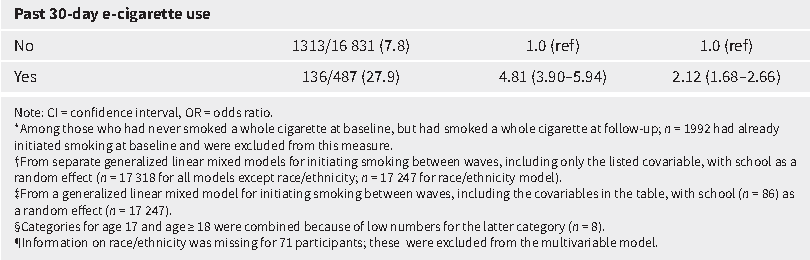
\includegraphics[width=0.5\textwidth]{3.pdf}
                  \caption{$ H_0 $: $ \theta_1\ge\theta_2 $ versus $ H_\text{A} $: $ \theta_1<\theta_2 $}{$ \mathcal{R}=\set{t\mid t\le -z_{\alpha}} $}
            \end{figure}
\end{itemize}
\begin{itemize}
      \item Defining Type I and Type II error rates in terms of a rejection region is also useful:
            \begin{itemize}
                  \item $ \alpha=\Prob*{\text{Type I Error}}=\Prob*{\text{Reject $ H_0 $}\given \text{$ H_0 $ is true}}=\Prob*{T\in\mathcal{R}\given \text{$ H_0 $ is true}} $.
                  \item $ \beta=\Prob*{\text{Type II Error}}=\Prob*{\text{Do Not Reject $ H_0 $}\given \text{$ H_0 $ is false}}=\Prob*{T\in\mathcal{R}^c\given \text{$ H_0 $ is false}} $.
            \end{itemize}
\end{itemize}
\begin{align*}
      1-\beta
       & =\text{Power}                                                                                                                                                                                                                                   \\
       & =1-\Prob*{\text{Type II Error}}                                                                                                                                                                                                                 \\
       & =1-\Prob*{T\in\mathcal{R}^c\given \text{$ H_0 $ is false}}                                                                                                                                                                                      \\
       & =\Prob*{T\in\mathcal{R}\given \text{$ H_0 $ is false}}                                                                                                                                                                                          \\
       & =\Prob*{T\ge z_{\alpha/2}\cup T\le -z_{\alpha/2}\given \text{$ H_0 $ is false}}                                                                                                                                                                 \\
       & =\Prob*{T\ge z_{\alpha/2}\given \text{$ H_0 $ is false}}+\Prob*{T\le -z_{\alpha/2}\given \text{$ H_0 $ is false}}                                                                                                                               \\
       & =\Prob*{\frac{\bar{Y}_1-\bar{Y}_2}{\sqrt{\frac{\Var{Y_1}+\Var{Y_2}}{n}}}\ge z_{\alpha/2}\given \text{$ H_0 $ is false}}+\Prob*{\frac{\bar{Y}_1-\bar{Y}_2}{\sqrt{\frac{\Var{Y_1}+\Var{Y_2}}{n}}}\le -z_{\alpha/2}\given \text{$ H_0 $ is false}}
\end{align*}
Assuming $ H_0 $ is true, $ \theta_1-\theta_2=0 $ and $ \displaystyle \frac{\bar{Y}_1-\bar{Y}_2}{\sqrt{\frac{\Var{Y_1}+\Var{Y_2}}{n}}} \sim \N{0,1} $.
However, $ H_0 $ is false, which means that $ \theta_1-\theta_2=\delta $ for some $ \delta\ne 0 $. Thus,
\[ \frac{\bigl(\bar{Y}_1-\bar{Y}_2\bigr)-\delta}{\sqrt{\frac{\Var{Y_1}+\Var{Y_2}}{n}}}\sim \N{0,1}  \]
Therefore, we need to account for this. Let $ Z \sim \N{0,1} $, then
\begin{align*}
      1-\beta
       & =\Prob*{\frac{\bigl(\bar{Y}_1-\bar{Y}_2\bigr)-\delta}{\sqrt{\frac{\Var{Y_1}+\Var{Y_2}}{n}}}\ge z_{\alpha/2}-\frac{\delta}{\sqrt{\frac{\Var{Y_1}+\Var{Y_2}}{n}}}}+\Prob*{\frac{\bigl(\bar{Y}_1-\bar{Y}_2\bigr)-\delta}{\sqrt{\frac{\Var{Y_1}+\Var{Y_2}}{n}}}\le -z_{\alpha/2}-\frac{\delta}{\sqrt{\frac{\Var{Y_1}+\Var{Y_2}}{n}}}} \\
       & =\Prob*{Z\ge z_{\alpha/2}-\frac{\delta}{\sqrt{\frac{\Var{Y_1}+\Var{Y_2}}{n}}}}+\Prob*{Z\le -z_{\alpha/2}-\frac{\delta}{\sqrt{\frac{\Var{Y_1}+\Var{Y_2}}{n}}}}
\end{align*}
Think about what happens to these terms when $ \delta $ is positive versus negative.
Without loss of generality, assume $ \delta>0 $, in which case
\[ 1-\beta=\Prob*{Z\ge z_{\alpha/2}-\frac{\delta}{\sqrt{\frac{\Var{Y_1}+\Var{Y_2}}{n}}}} \]
We know that $ \Prob*{Z\ge z_{1-\beta}}=1-\beta $, therefore
\[ z_{1-\beta}=z_{\alpha/2}-\frac{\delta}{\sqrt{\frac{\Var{Y_1}+\Var{Y_2}}{n}}} \]
Doing some algebra yields
\[ n=\frac{(z_{\alpha/2}-z_{1-\beta})^2\bigl[\Var{Y_1}+\Var{Y_2}\bigr]}{\delta^2}  \]
\begin{itemize}
      \item $ \Var{Y_1} $ and $ \Var{Y_2} $ are the variances of the response in the two conditions.
            This needs to be guessed or determined by historical information.
      \item $ \delta=\theta_1-\theta_2 $ is called the \textbf{minimum detectable effect} (MDE), and it
            is the smallest difference between $ \theta_1 $ and $ \theta_2 $ that has practical importance
            and that we would like to detect as being statistically significant.
\end{itemize}
